\lipsum[1]

\begin{figure}[H]
\centering
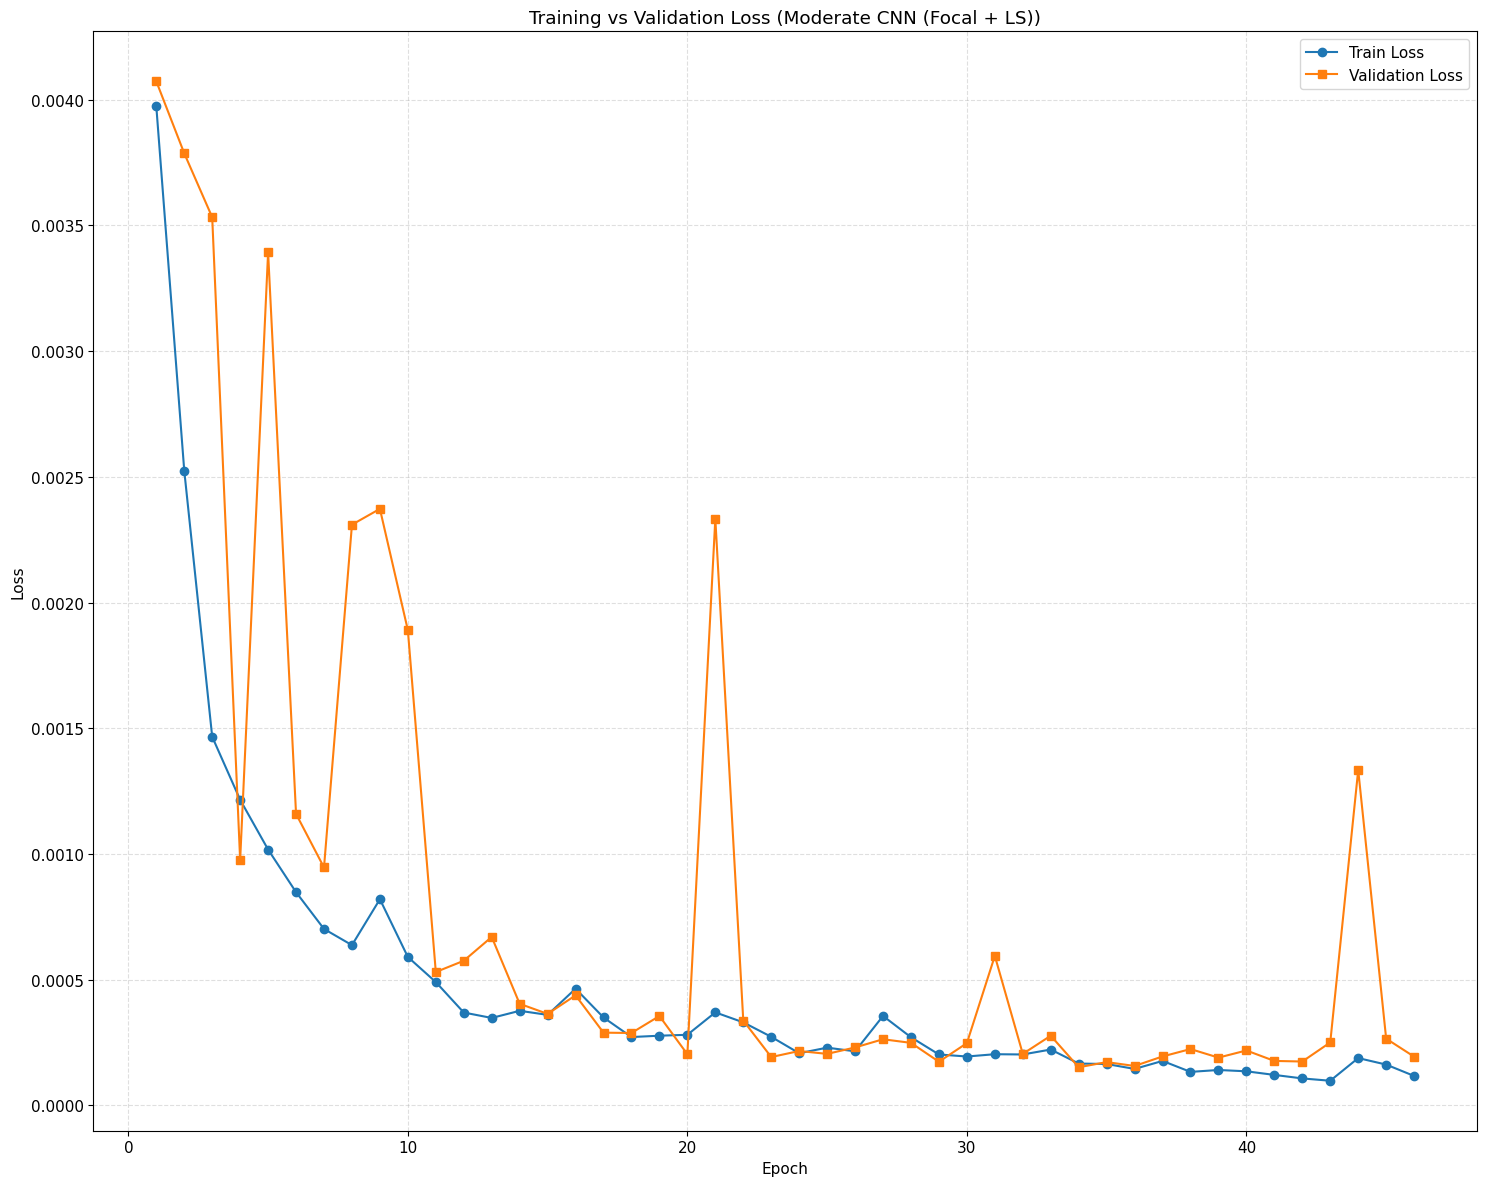
\includegraphics[width=\linewidth]{Figures/resultsfigures/image4.png}
\caption{Training and validation loss curves for the Moderate CNN trained with focal loss and label smoothing. The focal-loss objective introduces noticeable fluctuations in validation loss due to its strong emphasis on hard samples, resulting in less stable optimization compared to cross-entropy–based variants.}
\label{fig:focal-loss-curves}
\end{figure}

\begin{figure}[H]
\centering
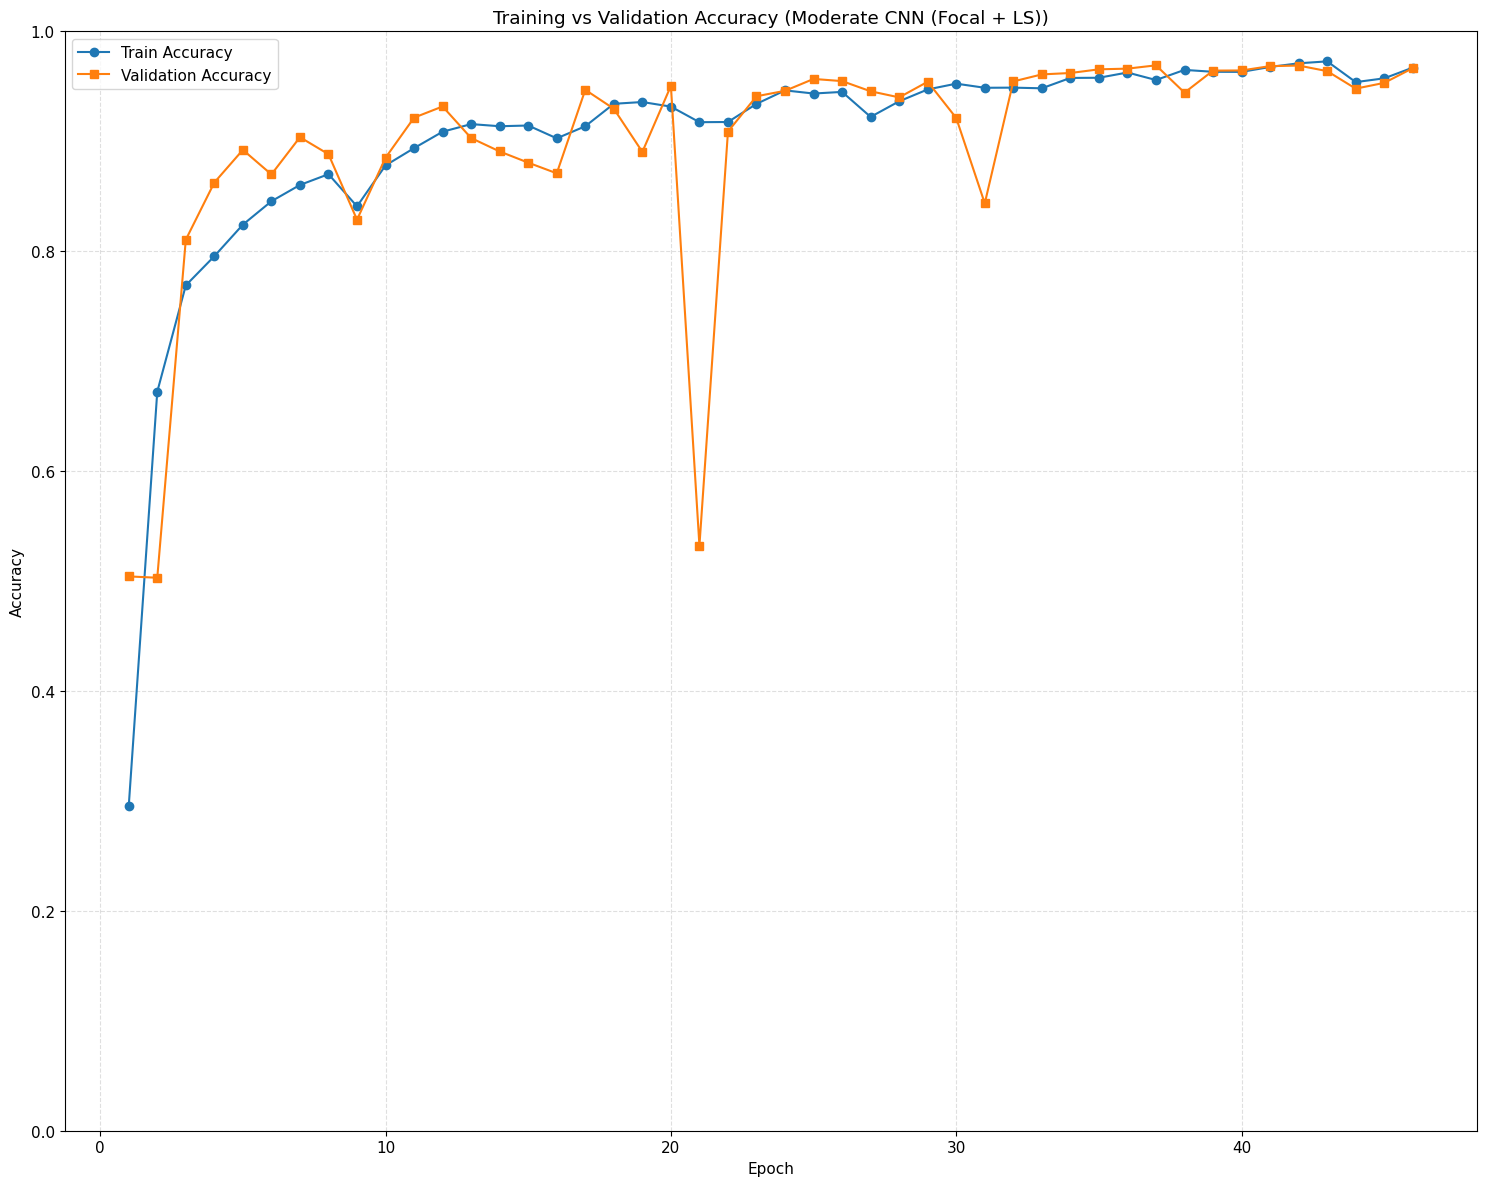
\includegraphics[width=\linewidth]{Figures/resultsfigures/image5.png}
\caption{Training and validation accuracy curves for the Moderate CNN trained with focal loss and label smoothing. Despite occasional validation drops, overall accuracy converges near 98\%, indicating strong generalization despite noisier optimization dynamics.}
\label{fig:focal-accuracy-curves}
\end{figure}

\textbf{Quantitative Results}
\begin{table}[htbp]
\centering
\caption{Overall performance metrics of the Moderate CNN trained with focal loss and label smoothing.}
\label{tab:focal-loss-metrics}

\begin{tabular}{|l|c|}
\hline
\textbf{Metric} & \textbf{Value} \\ \hline
Accuracy & 0.9424 \\ \hline
Macro Precision & 0.7982 \\ \hline
Macro Recall & 0.9590 \\ \hline
Macro F1 & 0.8280 \\ \hline
\end{tabular}

\end{table}


U2R recall remains perfect (1.0000), but precision collapses to 0.2204.

\textbf{Interpretation}  
Despite its popularity in computer vision tasks, focal loss is ill-suited for NSL-KDD’s extreme imbalance. It overcorrects for minority classes, leading to unstable training and reduced overall performance.

\subsection{Final Best Configuration: Weighted CE with Label Smoothing}
The final Moderate CNN model employs weighted cross-entropy combined with label smoothing.

\textbf{Numerical Summary}
\begin{table}[htbp]
\centering
\caption{Overall performance metrics of the final Moderate CNN model evaluated on the combined NSL-KDD test set.}
\label{tab:final-model-metrics}

\begin{tabular}{|l|c|}
\hline
\textbf{Metric} & \textbf{Value} \\ \hline
Accuracy & 0.9625 \\ \hline
Macro Precision & 0.8660 \\ \hline
Macro Recall & 0.9752 \\ \hline
Macro F1 & 0.9042 \\ \hline
\end{tabular}

\end{table}


\textbf{Per-class performance highlights:}
\begin{itemize}
    \item R2L F1 = 0.9534 with 0.9726 recall
    \item U2R F1 = 0.6802 with 1.0000 recall
    \item DoS and Probe F1 exceed 0.99 and 0.94, respectively
\end{itemize}

\textbf{Interpretation}  
This configuration delivers the best balance across all classes, the highest macro-F1, stable training dynamics, minimal overfitting, and high attack sensitivity without excessive false alarms. Weighted cross-entropy combined with label smoothing is therefore the optimal choice for NSL-KDD.

\subsection{Consolidated Ablation Summary}

\begin{table}[H]
\centering
\caption{Sensitivity of the Moderate CNN to Loss and Balancing Techniques}
\label{tab:ablation-summary}

\resizebox{\textwidth}{!}{%
\begin{tabular}{|l|c|c|c|c|c|c|c|c|}
\hline
\textbf{Configuration} & \textbf{CE} & \textbf{CW} & \textbf{LS} & \textbf{FL} & \textbf{Accuracy} & \textbf{Macro Prec.} & \textbf{Macro Rec.} & \textbf{Macro F1} \\ \hline
Standard CE (baseline) & T & F & F & F & $\sim$0.93--0.94 & Low & Low & Low \\ \hline
Weighted CE & T & T & F & F & $\sim$0.95--0.96 & Moderate & High & Good \\ \hline
Weighted CE + LS (Best) & T & T & 0.1 & F & 0.9625 & 0.8660 & 0.9752 & 0.9042 \\ \hline
Focal Loss + LS & F & F & 0.05 & T & 0.9436 & 0.8032 & 0.9577 & 0.8358 \\ \hline
\end{tabular}
}

\vspace{0.5em}
\noindent\textit{* T = True, F = False}
\end{table}

